\section{Auswertung}
\label{sec:Auswertung}

\subsection{Überprüfung der Stabilitätsbedingung}
\label{sec:stabil}

Die Stabilitätsbedingung aus Gleichung \eqref{eqn:stab} wird für zwei Kombinationen der Spiegel überprüft.
Als Auskopplungsspiegel wird ein Spiegel genutzt bei dem die reflektierende Fläche einen Krümmungsradius von $r = \SI{1400}{\milli\meter}$ besitzt. Der stark refelektierende Spiegel hat erst ebenfalls einen Krümmungsradius von $r = \SI{1400}{\milli\meter}$ und wird dann in der zweiten überprüften Kombination durch einen flachen Spiegel ersetzt.
Die theoretisch erreichbare maximale Länge $L$ des Resonators kann in Abbildung \ref{fig:stabil} abgelesen werden. Wie auch in Formel \eqref{eqn:stab} zu erkennen ist, liegt diese bei zwei krummen Spiegeln bei $r_1+r_2$ und bei der zweiten Kombination bei $r_1$.

\begin{figure}
  \centering
  \includegraphics[height=9cm]{build/stabil.pdf}
  \caption{Die theoretisch erreichbaren Verstärkungsfaktoren der beiden Spiegelkombinationen. }
  \label{fig:stabil}
\end{figure}

Die experimentell erreichten maximalen Resonatorlängen sind in Tabelle \ref{tab:stabil} zu sehen.

\begin{table}
  \centering
  \begin{tabular}{l l S}
    \toprule
    {HR-Spiegel}& {OC-Spiegel} & {$L_\text{max}\:/\:\si{\centi\meter}$}\\
    \midrule
    $r = \SI{1400}{\milli\meter}$/flat & $r = \SI{1400}{\milli\meter}$/flat & 215.4\\
    flat/flat & $r = \SI{1400}{\milli\meter}$/flat & 126.5\\
    \bottomrule
  \end{tabular}
  \caption{Die erreichten maximalen Resonatorlängen.}
  \label{tab:stabil}
\end{table}

\subsection{Vermessung der TEM-Moden}

\paragraph{TEM$_{00}$ Grundmode}

Die gemessene Intensität der TEM$_{00}$ Grundmode in Abhängigkeit der Position der Photodiode ist in Tabelle \ref{tab:grundmode} eingetragen.

\begin{table}
  \centering
  \begin{tabular}[t]{S S}
    \toprule
    {$x\:/\:\si{\milli\meter}$} & {$I\:/\:\si{\micro\ampere}$}\\
    \midrule
    28 & 0.22\\
    25 & 0.512\\
    22 & 0.96\\
    19 & 1.593\\
    16 & 2.375\\
    13 & 2.946\\
    \bottomrule
  \end{tabular}
  \begin{tabular}[t]{S S}
    \toprule
    {$x\:/\:\si{\milli\meter}$} & {$I\:/\:\si{\micro\ampere}$}\\
    \midrule
    10 & 2.971\\
    7 & 2.489\\
    4 & 1.78\\
    1 & 1.152\\
    -2 & 0.667\\
    -5 & 0.386\\
    -8 & 0.181\\
    \bottomrule
  \end{tabular}
  \caption{Messwerte der Intensitätsverteilung der TEM$_{00}$ Grundmode mit den Unsicherheiten $\sigma_x = \SI{0.5}{\milli\meter}$ und $\sigma_I = \SI{0.01}{\micro\ampere}$.}
  \label{tab:grundmode}
\end{table}

An diese Messwerte wurde die Funktion
\begin{align}
  I = I_0*\exp((-2*(x+x_0)^2)/(\omega^2))
\end{align}
gefittet. Es ergeben sich die Werte:
\begin{align}
  I_0 = \SI{1.25(3)}{\micro\ampere} \quad x_0 = \SI{-11.1(1)}{\milli\meter} \quad \omega = \SI{14.7(2)}{\milli\meter}.
\end{align}
Die Messwerte und die Fitfunktion sind in Abbildung \ref{fig:grundmode} zu sehen.

\begin{figure}
  \centering
  \includegraphics[height=8cm]{build/grundmode.pdf}
  \caption{Messwerte und Fitfunktion für die TEM$_{00}$ Grundmode.}
  \label{fig:grundmode}
\end{figure}

\paragraph{TEM$_{01}$ Mode}

Die gemessene Intensität der TEM$_{01}$ Mode in Abhängigkeit der Position der Photodiode ist in Tabelle \ref{tab:transmode} eingetragen.

\begin{table}
  \centering
  \begin{tabular}[t]{S S}
    \toprule
    {$x\:/\:\si{\milli\meter}$} & {$I\:/\:\si{\micro\ampere}$}\\
    \midrule
    -10 & 0.018\\
    -8 & 0.044\\
    -6 & 0.052\\
    -4 & 0.066\\
    -2 & 0.065\\
    0 & 0.072\\
    2 & 0.105\\
    4 & 0.132\\
    6 & 0.108\\
    8 & 0.125\\
    10 & 0.101\\
    \bottomrule
  \end{tabular}
  \begin{tabular}[t]{S S}
    \toprule
    {$x\:/\:\si{\milli\meter}$} & {$I\:/\:\si{\micro\ampere}$}\\
    \midrule
    12 & 0.069\\
    14 & 0.036\\
    16 & 0.013\\
    18 & 0.001\\
    20 & 0.006\\
    22 & 0.023\\
    24 & 0.043\\
    26 & 0.065\\
    28 & 0.071\\
    30 & 0.053\\
    32 & 0.052\\
    34 & 0.041\\
    \bottomrule
  \end{tabular}
  \caption{Messwerte der Intensitätsverteilung der TEM$_{01}$ Mode mit den Unsicherheiten $\sigma_x = \SI{0.5}{\milli\meter}$ und $\sigma_I = \SI{0.01}{\micro\ampere}$.}
  \label{tab:transmode}
\end{table}

An diese Messwerte wurde die Funktion
\begin{align}
  %I = I_{0,1}*\exp((-2*(x+x_{0,1})^2)/(\omega_1^2)) + I_{0,2}*\exp((-2*(x+x_{0,2})^2)/(\omega_2^2))
  I = I_0 (x-x_0)^2 \exp\left[-2\left(\frac{x-x_0}{\omega}\right)^2\right]
\end{align}
gefittet. Es ergeben sich die Werte:
\begin{align}
  I_0 = \SI{1.3(1)}{\nano\ampere} \quad x_{0} = \SI{20.3(6)}{\milli\meter} \quad \omega = \SI{22(1)}{\milli\meter}
  %I_{0,2} = \SI{71(10)}{\nano\ampere} \quad x_{0,2} = \SI{-28.2(7)}{\milli\meter} \quad \omega_2 = \SI{7(2)}{\milli\meter}
\end{align}
Die Messwerte und die Fitfunktion sind in Abbildung \ref{fig:transmode} zu sehen.

\begin{figure}
  \centering
  \includegraphics[height=8cm]{build/transmode.pdf}
  \caption{Messwerte und Fitfunktion für die TEM$_{01}$ Mode.}
  \label{fig:transmode}
\end{figure}

\subsection{Polarisationsmessung}

Die Messwerte der Polarisationsmessung sind in Tabelle \ref{tab:polarisation} zu finden.
\begin{table}
  \centering
  \begin{tabular}[t]{S S}
    \toprule
    {$\phi\:/\:\si{\degree}$} & {$I\:/\:\si{\micro\ampere}$}\\
    \midrule
    0 & 0.65\\
  10 & 0.51\\
  20 & 0.38\\
  30 & 0.25\\
  40 & 0.08\\
  50 & 0.0\\
  60 & 0.03\\
  70 & 0.15\\
  80 & 0.4\\
    \bottomrule
  \end{tabular}
  \begin{tabular}[t]{S S}
    \toprule
    {$\phi\:/\:\si{\degree}$} & {$I\:/\:\si{\micro\ampere}$}\\
    \midrule
    90 & 0.64\\
    100 & 0.93\\
    110 & 1.09\\
    120 & 1.25\\
    130 & 1.3\\
    140 & 1.24\\
    150 & 0.98\\
    160 & 0.85\\
    170 & 0.73\\
    180 & 0.61\\
    \bottomrule
  \end{tabular}
  \caption{Messwerte der Polarisationsmessung.}
  \label{tab:polarisation}
\end{table}

An die Messwerte wird dann die Funktion
\begin{align}
  I = I_0\cos^2(m\phi + \phi_0)
\end{align}
gefittet. Wobei $\phi$ in Radian umgerechnet wird.

Es ergeben sich die Werte:
\begin{align}
  I_0 = \SI{1.25(3)}{\micro\ampere} \quad \phi_0 = \SI{0.67(3)}{\radian} \quad m = \num{1.01(2)}.
\end{align}

\begin{figure}
  \centering
  \includegraphics[height=8cm]{build/polarisation.pdf}
  \caption{Messwerte und Fitfunktion bei der Messung der Polarisation.}
  \label{fig:polarisation}
\end{figure}

\subsection{Wellenlängenmessung}
\label{sec:wellenlaenge}

Zur Bestimmung der Wellenlänge aus den Abständen der Beugungsmuster zur Mitte $d_\text{n}$ wird die Formel
\begin{align}
  \lambda = \frac{g \sin\left[\arctan\left(\frac{d_\text{n}}{L}\right)\right]}{n}
\end{align}
 verwendet. Sie folgt aus der Bragg-Bedingung
Der Abstand von Gitter zum Schirm $L$ und die Gitterkonstante $g$ betragen:
\begin{align}
  L = \SI{79.8(5)} \qquad g = \SI{12.5}{\micro\meter}.
\end{align}
Die Abstände der Nebenmaxima vom Hauptmaximum des Musters und die zugehörige Ordnung sind in Tabelle \ref{tab:wellenlaenge} zu finden. Dort findet sich auch die jeweils berechnete Wellenlänge mit Unsicherheit. Da links und rechts vom Hauptmaximum gemessen wurde, tritt jede Ordnung zwei mal auf.
\begin{table}[h]
  \centering
  \begin{tabular}{S S
    S[table-format=3.0]
    @{${}\pm{}$}
    S[table-format=2.0]
     }
    \toprule
    {$d_\text{n}\:/\:\si{\centi\meter}$} &{$n$}& \multicolumn{2}{c}{$\lambda\:/\:\si{\nano\meter}$}\\
    \midrule
    3.8 & 1 & 594 & 31\\
    7.8 & 2 & 608 & 22\\
    11.9 & 3 & 614 & 17\\
    15.9 & 4 & 610 & 15\\
    20.1 & 5 & 610 & 13\\
    24.6 & 6 & 613 & 11\\
    3.8 & 1 & 594 & 31\\
    7.9 & 2 & 615 & 22\\
    11.9 & 3 & 614 & 17\\
    16.1 & 4 & 618 & 15\\
    20.4 & 5 & 619 & 13\\
    24.8 & 6 & 618 & 11\\
    \bottomrule
  \end{tabular}
  \caption{Die Messwerte und Ergebnisse aus der Messung der Wellenlänge. Der Fehler der Abstände wird auf $\sigma_\text{d} = \SI{0.2}{\centi\meter}$ angenommen.}
  \label{tab:wellenlaenge}
\end{table}
Mit den Werten aus Tabelle \ref{tab:wellenlaenge} wird für die Wellenlänge der Mittelwert
\begin{align}
  \lambda = \SI{611(12)}{\nano\meter}
\end{align}
berechnet. Das entspricht einer Abweichung vom erwarteten Wert $\lambda_\text{erw.} = \SI{632.8}{\nano\meter}$ von $\SI{3(2)}{\percent}$.

\subsection{Longitudinale Moden}

Aus den Frequenzen der stehenden Wellen zwischen den Resonatorspiegeln wird nun die Distanz der beiden Spiegel bestimmt. Die vier für jede Distanz aufgenommenen Frequenzen sind in Tabelle \ref{tab:longiModen} zu finden. Dass die Schwebung mehrerer Frequenzen auftreten kann, folgt aus der gaußförmigen Einhüllenden der Kammzinken der Emissionslinie \cite{longimodenText}.
Dargestellt ist dies in Abbildung \ref{fig:LaserModes}. Im Fall von Neon soll die Breite des Peaks abgeschätzt werden. Dass die Emissionslinie keine scharfe Linie ist, liegt an der Dopplerverbreiterung aufgrund der thermalen Bewegung der Neonatome. Nach \cite{thermal} ist die thermale Geschwindigkeit von Neon als Effektivwert in drei Dimensionen $v_\text{3D, eff.} = \SI{602}{\meter\per\second}$. Dort wird die Formel
\begin{align}
  v_\text{3D, eff.} = \sqrt{\frac{3 k_\text{B} T}{m}}
\end{align}
benutzt, wobei $k_\text{B}$ die Boltzmannkonstante, $T$ die Temperatur ist und $m$ die Masse eines Neonatoms. Zur Umrechnung in eine Dimension muss also noch durch $\sqrt{3}$ geteilt werden. Wenn dieser Wert dann in die Formel für Dopplerverbreiterung:
\begin{align}
  f_\text{gemessen} = f_\text{Neon} \frac{c}{c - v_\text{1D, eff.}}
\end{align}
eingesetzt wird, kann die Breite des Gauss durch
\begin{align*}
  \delta_\text{f} &= 2 (f_\text{gemessen} - f_\text{Neon})
                  \quad = 2 (\SI{473.744035}{\tera\hertz} - \SI{473.743486}{\tera\hertz})\\
                  &= \SI{1098}{\mega\hertz}
\end{align*}
abgeschätzt werden. Dabei ist $f_\text{Neon}$ die Frequenz, der theoretischen Emissionslinie von Neon. Da $\delta_\text{f}$ also größer ist als die Frequenzdifferenzen der longitudinalen Moden, die von der Länge des Resonators bestimmt werden, können mehrere Moden verstärkt werden und die Schwebung so entstehen.
\begin{figure}
  \centering
  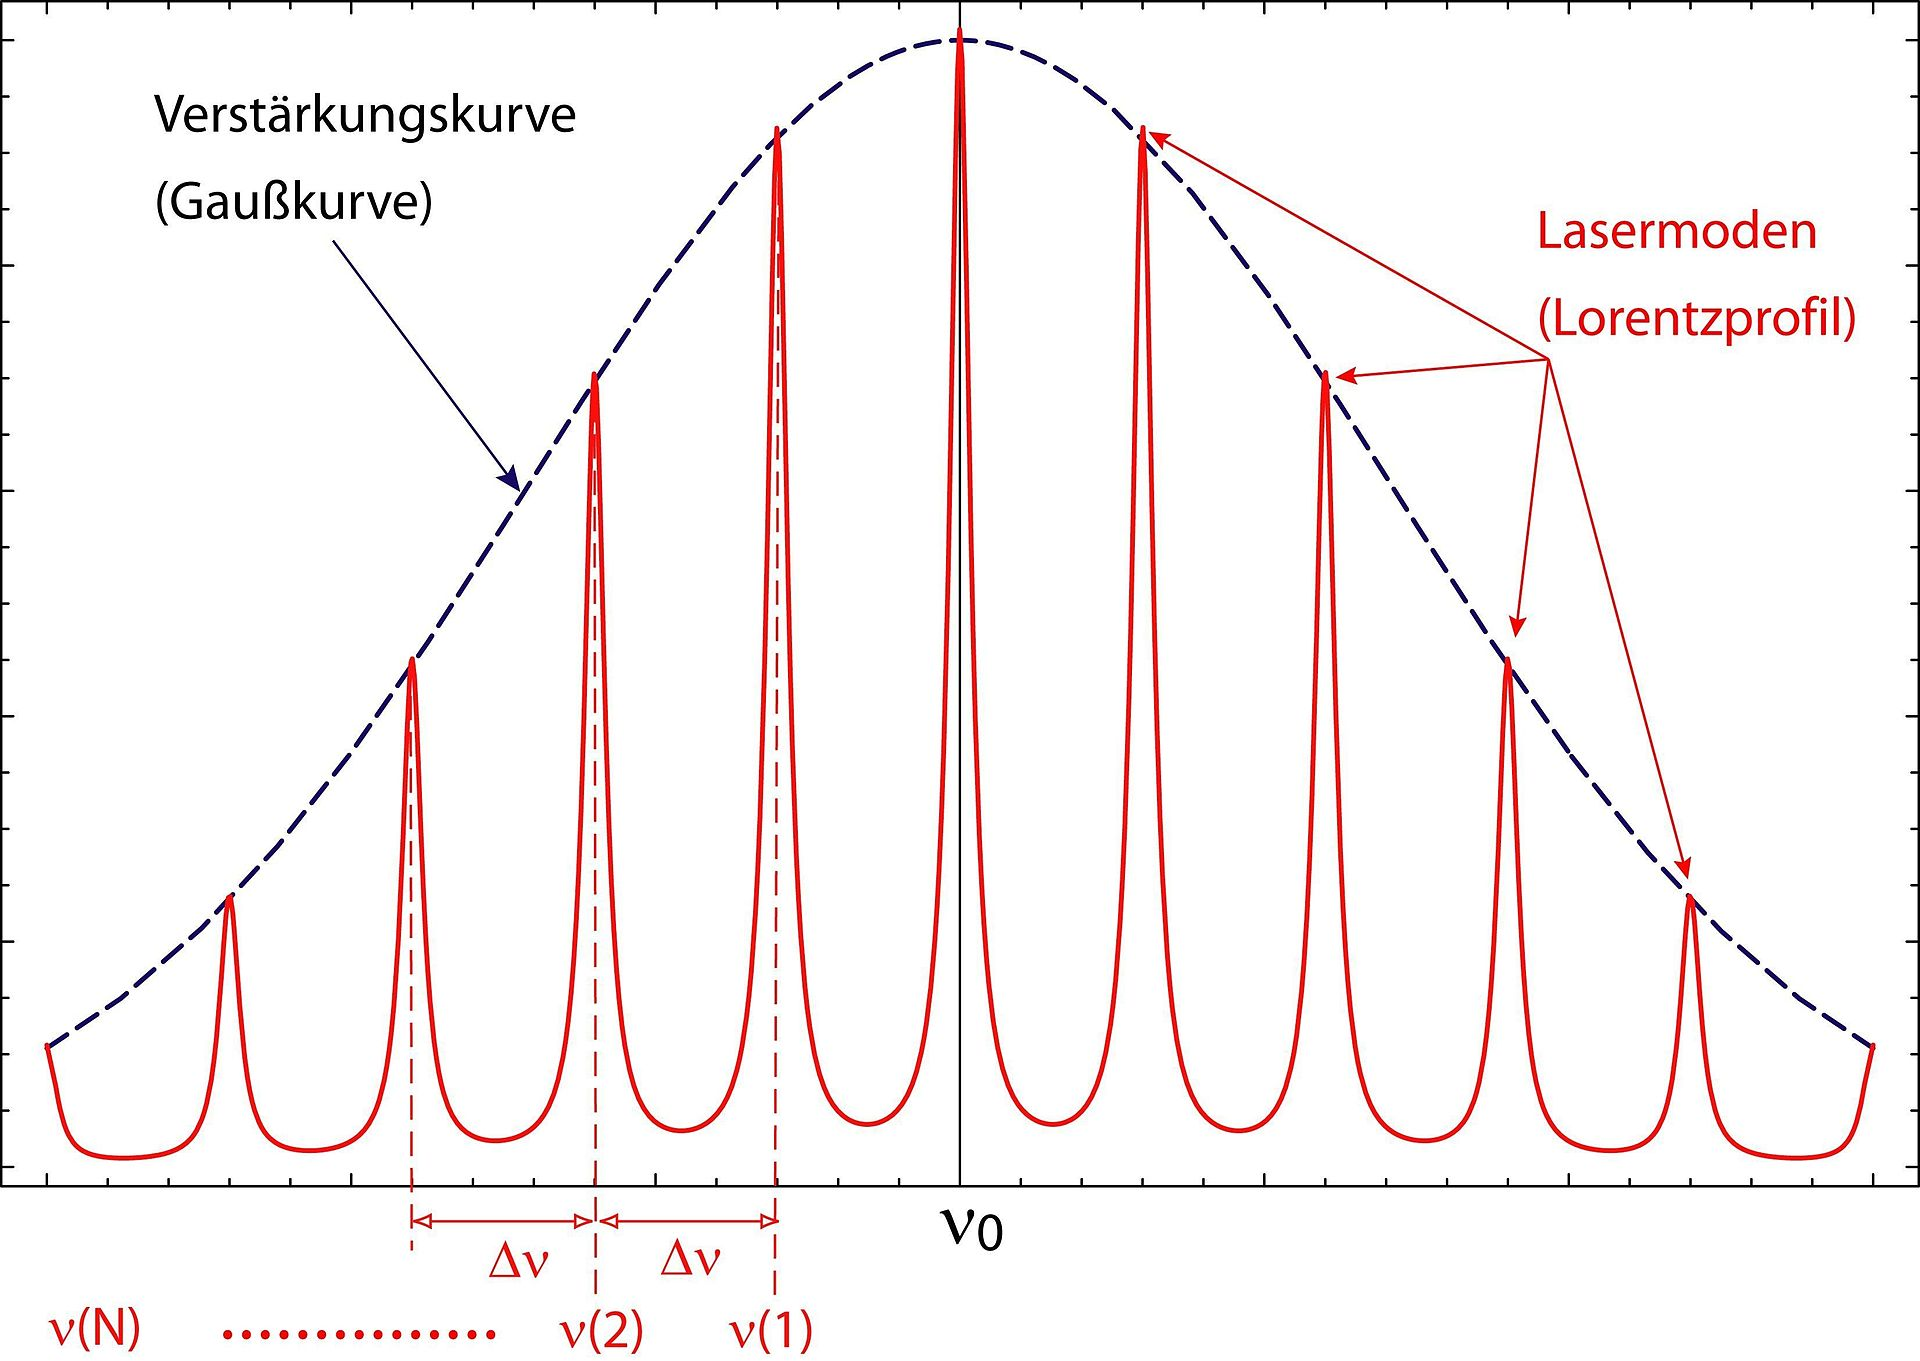
\includegraphics[height=8cm]{Pics von Buddy/LaserModes.jpg}
  \caption{Longitudinale Lasermoden bei gaußförmigem Verstärkungsprofil in einem Resonator. Darstellung: Amplitude als Funktion der Frequenz \cite{longimodenBild}.}
  \label{fig:LaserModes}
\end{figure}

\begin{table}
  \centering
  \begin{tabular}{S}
    \toprule
    {$\nu_{1, L = \SI{53.5}{\centi\meter}}\:/\:\si{\mega\hertz}$}\\
    \midrule
    278\\
551\\
825\\
1099\\
    \bottomrule
  \end{tabular}
  \begin{tabular}{S}
    \toprule
    {$\nu_{2, L = \SI{60.5}{\centi\meter}}\:/\:\si{\mega\hertz}$}\\
    \midrule
244\\
488\\
728\\
971\\
    \bottomrule
  \end{tabular}
  \begin{tabular}{S}
    \toprule
    {$\nu_{3, L = \SI{75.6}{\centi\meter}}\:/\:\si{\mega\hertz}$}\\
    \midrule
203\\
405\\
611\\
814\\
    \bottomrule
  \end{tabular}
  \caption{Messwerte der Frequenzmessung bei unterschiedlichen Resonatorlängen. Als Fehler der Frequenzmessung wird $\sigma_{\nu} = \SI{5}{\mega\hertz}$ angenommen.}
  \label{tab:longiModen}
\end{table}

Daraus wird mit Formel \eqref{eqn:freqabstand} die Länge des Resonators berechnet. Dazu werden die vier Frequenzdifferenzen pro Resonatorlänge gemittelt. Die Ergebnisse, sowie die mit Bandmaß gemessene Resonatorlänge und die Abweichung davon sind in Tabelle \ref{tab:longiModenErgebnisse}.

\begin{table}[h]
  \centering
  \begin{tabular}{S[table-format=2.1]
      @{${}\pm{}$}
      S[table-format=1.1] S S[table-format=1.0]
      @{${}\pm{}$}
      S[table-format=1.0]}
    \toprule
    \multicolumn{2}{c}{$L_\text{ber.}\:/\:\si{\centi\meter}$} & {$L_\text{gem.}\:/\:\si{\centi\meter}$} & \multicolumn{2}{c}{$\Delta\:/\:\si{\percent}$}\\
    \midrule
    54.6 & 0.2 & 53.5 & 2 & 1\\
    61.8 & 0.3 & 60.5 & 2 & 1\\
    73.7 & 0.5 & 75.6 & 3 & 1\\
    \bottomrule
  \end{tabular}
  \caption{Die Ergebnisse der Ausmessung der longitudinalen Moden. Als Fehler der Bandmassmessung wird $\sigma_{L_\text{gem.}} = \SI{0.5}{\centi\meter}$ angenommen.}
  \label{tab:longiModenErgebnisse}
\end{table}






% \begin{figure}
%   \centering
%   \includegraphics[height=5cm]{build/plotElement.pdf}
%   \caption{Plot.}
%   \label{fig:plot}
% \end{figure}
%
% Tabelle für copy and paste:
% \begin{table}[h]
%   \centering
%   \begin{tabular}{S S}
%     \toprule
%     {$k$} & {$U\:/\:\si{\milli\volt}$}\\
%     \midrule
%     1 & 637.2\\
%     3 & 212.4\\
%     5 & 127.4\\
%     7 & 91.03\\
%     9 & 70.8\\
%     \bottomrule
%   \end{tabular}
%   \caption{Amplituden Rechteckspannung.}
%   \label{tab:rechtampl}
% \end{table}
